\section{Testing and Verification}
\begin{itemize}
\item Verification: is the program right (correct)?
\item Validation: is the right program (what the client wants)?
\end{itemize}

Everything must be verified (specifications, design, test data etc.) along the entire development process.

Failures are usually result of faults introduced by human error.\\
Human Error → System fault → System failure

Verification and validation start as soon we decide to develop a product, design must permit testing of the system.

Difficulties:
\begin{itemize}
    \item Impossible to develop error free software
    \item Properties may bu subjective
    \item Properties may be implicit or not clearly stated
    \item Goals not reasonable
\end{itemize}

\subsection{Verification model}
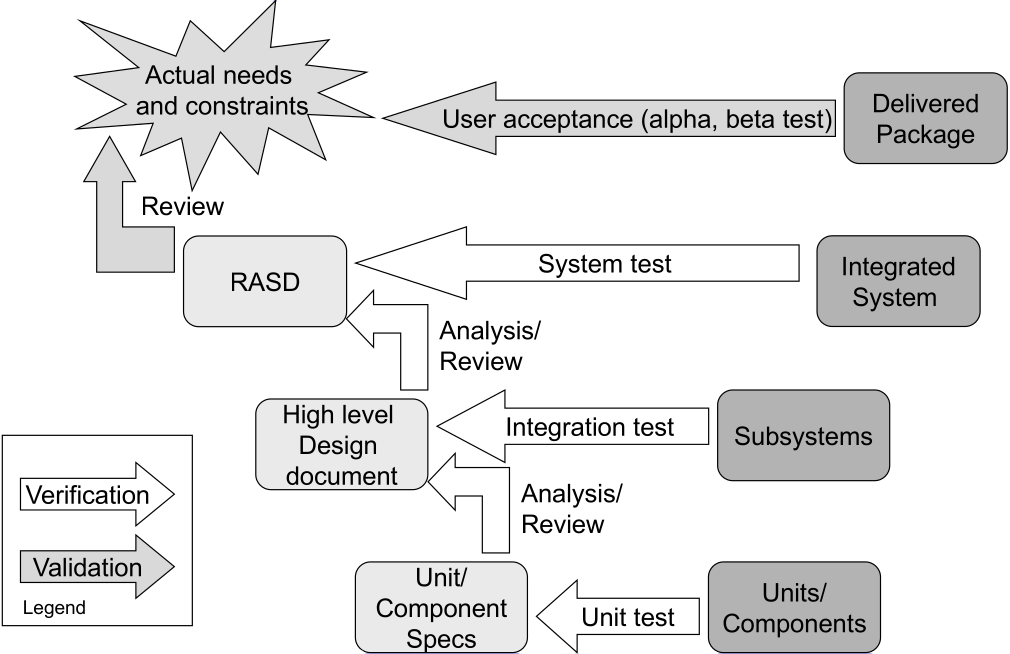
\includegraphics[width=\linewidth]{7-testing/v-model.png}

\section{Analysis}
Software is not executed, so analysis can be made even at early stages when software cannot be executable (yet).
The two main approaches are (manual) inspection and automated static analysis.

\subsection{Review, Walkthrough, Inspection}
Formal evaluation in which software (or plans, design, documentation, everything) is examined to find faults, violations of standards etc.

Objective is finding errors in the product, not fixing them or evaulting the producer.

\textbf{Walkthrough}
Producer presents product and the reviewers comment on the correctness and consistency.
\begin{itemize}
    \item Informal review
    \item Reviewers are experts in the domain
    \item Subject is correctness of product from POV of experts
    \item Leader of discussion/session controller is the producer
\end{itemize}

\textbf{Inspection}
\begin{itemize}
    \item Formal review
    \item Reviewers are trained, professional inspectors
    \item Subject is correctness of product according to given checklist
    \item Leader of discussion/session controller is official moderator of review team
\end{itemize}
Various roles:
\begin{itemize}
    \item Moderator: plans meeting, chooses participants, controls all the process
    \item Readers and testers (inspectors): read code and look for flaws
    \item Author: passive, only answer to questions
    \item Scribe (recorder)
\end{itemize}
Session are at most 2 hours, max 150 lines per hour.
Defects are only logged, not fixed.

\textbf{Modern code review}
Code visible to everyone, review facilitated by various tools.
Helps in exchanging and recording ideas.

\subsection{Static Analysis}
Based on identification of pairs of variables definitions and use.
Typically used by compilers to check for possible errors and to make optimizations.
Pessimistic approach, some problems may actually be false positives.
\begin{enumerate}
    \item Derive control flow graph
    \item Derive def and use sets for every node
    \item Identify pairs of def-use
\end{enumerate}

Can be used to check if variable is guaranteed to be initialized or if variable is never used.

\textbf{Symbolic execution}
Values are expressed over symbols, executing statements computes new expressions.
In case of branches, execution is performed only for a specified path.

\section{Testing}
\textbf{Test case} is a set of inputs of the system, along with the expected outcome (given hypothesis on state of the system).
\textbf{Test set} is a set of test cases.

Test cases can be generate randomly or systematically.

\subsection{Unit testing}
Conducted directly by the developers on single units of code.
Component may not work in isolation, so \emph{drivers} and \emph{stubs} are needed (this is called \textbf{scaffolding}).
Unit testing should be done as soon as possible.

\subsection{Integration testing}
Aimed to test interfaces and modules interactions.
Example of integration faults are:
\begin{itemize}
    \item Inconsistent interpretation of parameters
    \item Violations of capacity or size limits
    \item Side effects on resources
    \item Omitted or misunderstood functionality
    \item Nonfunctional properties (e.g. performance issues)
    \item Dynamic mismatches
\end{itemize}
Integration plan is an important part of the test plan, which is part of the project plan.

\textbf{Big Bang testing}\\
All integration testing done at the end, no scaffolding required.
Very bad, it has an high cost of repair (bugs found early cost less to be fixed).

\textbf{Incremental testing}\\
Integration testing is done while component are released, even at early stages.

\subsection{Testing strategies}
\begin{itemize}
    \item Top-down (requires stubs)
    \item Bottom-up (requires drivers)
    \item Thread (develop one function at a time)
    \item Critical modules (start by riskier modules, to verify feasibility)
\end{itemize}

\subsection{System testing}
Testing of the whole system, both functional and non-functional.
\begin{itemize}
    \item Performance testing (identify bottlenecks and benchmarking)
    \item Load testing (expose bugs such as memory leaks, identify upper limits of components)
    \item Stress testing (see how the system behaves in case of failures or sudden change of load and resources)
\end{itemize}

\subsection{Testing techniques}
\textbf{White box} Used usually for unit testing, based on knowledge of structure of the system.

\textbf{Black box} Used to test integration and the whole system. Used to check if expected behavior is the behavior of the software (\emph{Model-based testing}).

\textbf{Capture and reply} First test is manual (so it is costly) but it is recorded. Next time the test is an automatic replay of the first test, for which we know the outcome (used for example for auto-regression testing on GUI).

\subsection{Black box testing a state machine}
If the system acts like a state machine (there are states and transactions between them) there are 2 criterion of coverage:
\begin{itemize}
    \item Coverage of States: the test cases must collectively reach all the states
    \item Coverage of Transactions: the test cases must collectively reach all the transactions
\end{itemize}
